\smsection{Implementation}
\smvertspace
We implemented our analyses for the ES\&S iVotronic voting terminals
and built a web application in order for election officials and
advocacy groups to have easy access to our tool. The website requires
that the user uploads an event log and a ballot images file; we strongly
suggest they also submit the system log to take advantage of the
full range of analyses our tool provides.  The following describes how
our tool works.   

\begin{enumerate}
\item
The election is performed on DRE machines; Figure~\ref{fig:subfig1} shows the ES\&S iVotronic voting machine.  Event logs, ballot images files, and system logs are produced after each election.
\item
Election officials upload these files to AuditBear.  This web application is found at www.audit-bear.org, as displayed in Figure~\ref{fig:subfig2}.  
\item
AuditBear produces reports.  Figure~\ref{fig:subfig3} is an example of
one such report, titled ``PEBs Not Uploaded.'' From these reports,
election officials are 
warned about possible miscounts or procedural errors.  
\end{enumerate}

\begin{figure}[h]
\centering
\mbox{
\subfigure[iVotronic Machine]{
	\epsfig{figure=machine.png,width=1in}
	\label{fig:subfig1}}
\subfigure[audit-bear.org]{
	\epsfig{figure=indexpage.png,width=1in}
	\label{fig:subfig2}}
\subfigure[Reports]{
	\epsfig{figure=report2.png,width=1in}
	\label{fig:subfig3}}}
\caption{Workflow of AuditBear}
\label{auditBear}
\end{figure}

%\begin{figure}
%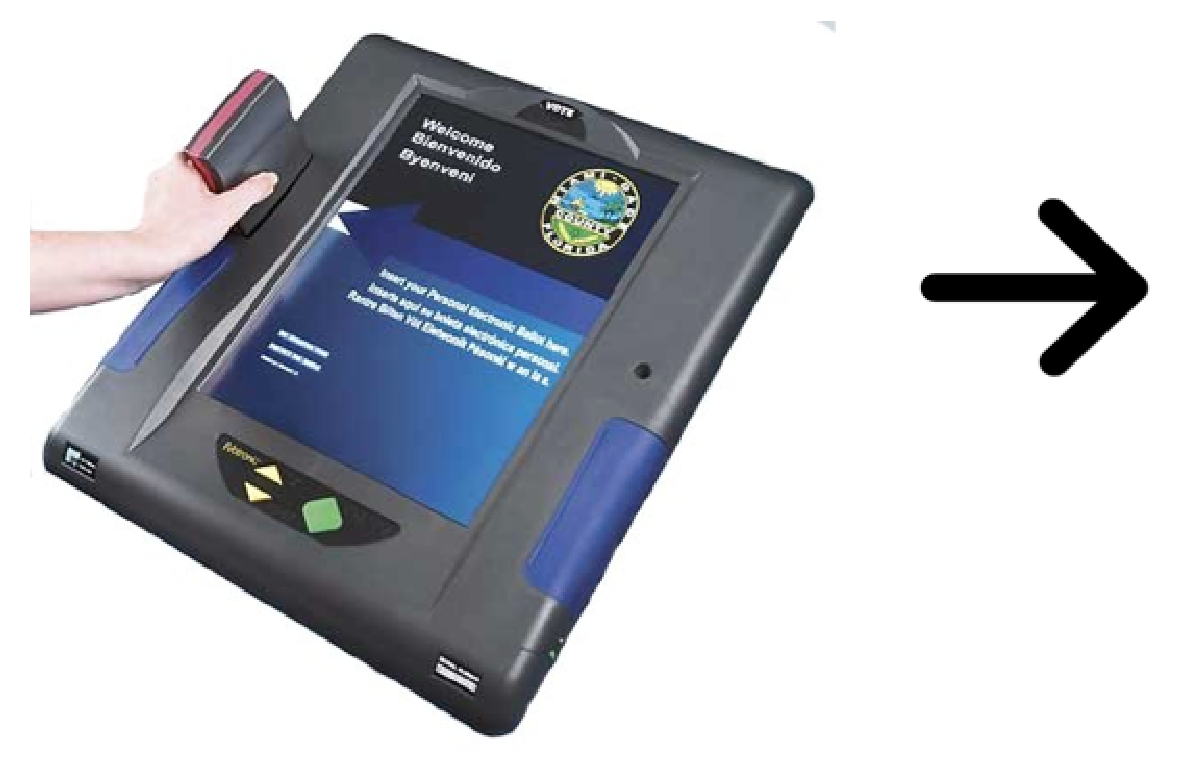
\includegraphics[scale=0.10]{machine.eps}
%\end{figure}
%\begin{figure}
%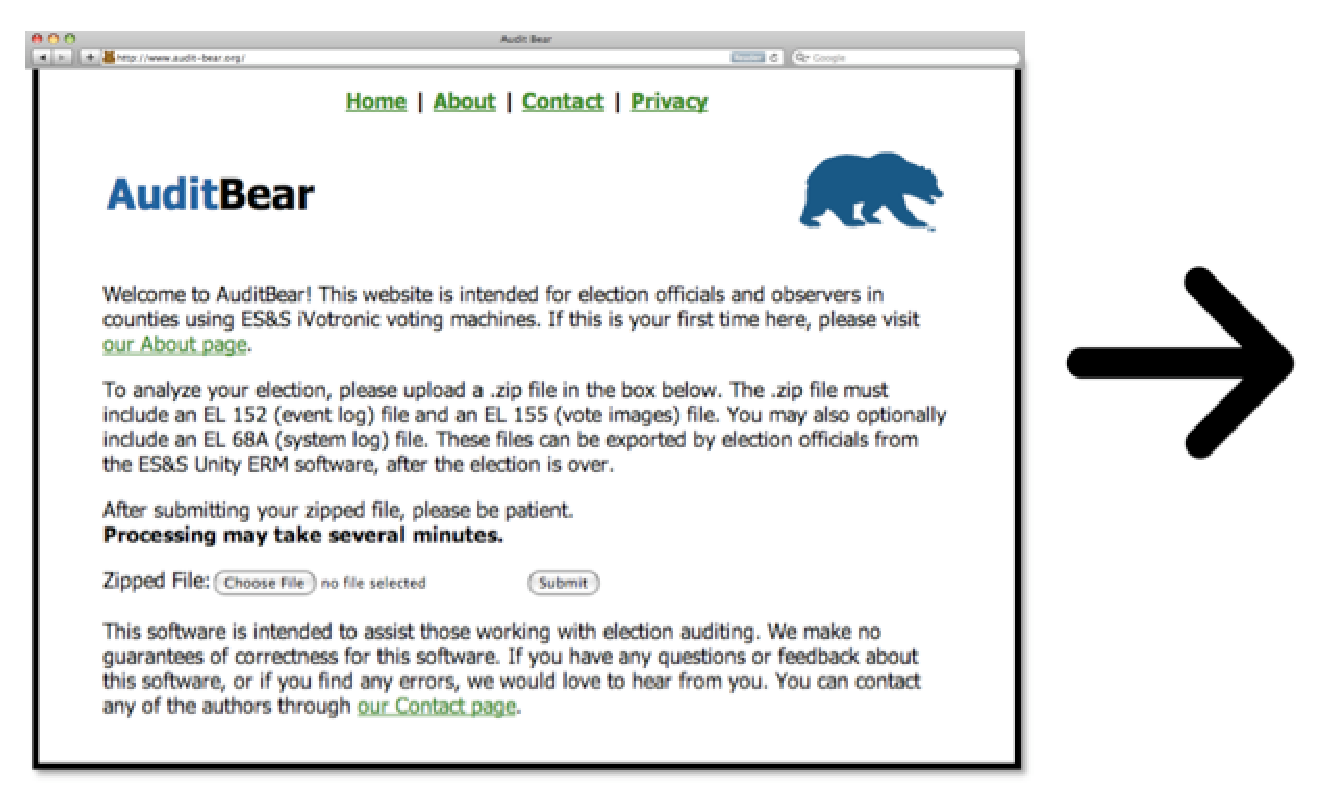
\includegraphics[scale=0.10]{indexpage.eps}
%\end{figure}
%\begin{figure}
%
\includegraphics[scale=0.10]{report.eps}
%\end{figure}

There are 15 possible reports generated by our tool, one
for each analysis described in Section \ref{sec:analysis}. \cks{Is 15
  the right number? I am sort of guessing.} However, a report is only
displayed if the analysis returns positive results. If a particular
analysis uncovers no anomalies in the audit logs, there is no need to display the
corresponding report. Each report that is displayed will give details
about the errors found and will
also explain the possible consequences of the error and suggest, where
applicable, steps the election officials might take to address
the error. To help the user focus on the most relevant information, we
ordered the reports so the most serious errors (i.e., those that might
result in votes being left out of the official tally) are at the top
and errors with less dire consequences are listed farther down. 

\smsubsection{Sample Reports}
\smvertspace

The following are sample reports generated by running AuditBear on the
audit data from the South Carolina 2010 General Election. 

Figure
\ref{fig:sample2} is an example of a report generated by the analysis
explained in Section \ref{sec:pebs_not_uploaded}. The report lists all
the PEBs that were used to close a machine, but whose data was not
uploaded to the election reporting 
system. In addition to giving the polling location and PEB serial
number, the report explains the possible consequences of this
error and suggests actions the election officials might take to
remedy the situation.
% \caption{This report displays the PEBs that were not uploaded in Greenville County.}
\begin{figure}[h]
\centering
\mbox{
\subfigure[PEBs not uploaded, Greenville Co.]{
  \label{fig:sample2}
    \includegraphics[width=0.5\textwidth]{sample3}
}
\subfigure[Opening and closing with different PEBs, Colleton Co.]{
  \label{fig:sample3}
    \includegraphics[width=0.5\textwidth]{sample2}
}
}
\end{figure}

Figure \ref{fig:sample3} is an example of a report generated by the
analysis described in Section \ref{sec:opening_closing_diff_pebs}. The
report lists all the machines that were not opened and closed by the
same PEB. This error occurs as a result of procedural error and the
report suggests election officials review their poll worker training
program.

%\begin{figure}[h!]
%  \caption{This report shows the machines that were opened and closed with different PEBs in Colleton County.}

%  \centering

%\end{figure}
